\section{CSC Trigonometric Cosecant Function}

\subsection{Usage}

Computes the \verb|csc| function for its argument.  The general
syntax for its use is
\begin{verbatim}
  y = csc(x)
\end{verbatim}
where \verb|x| is an \verb|n|-dimensional array of numerical type.
Integer types are promoted to the \verb|double| type prior to
calculation of the \verb|csc| function.  Output \verb|y| is of the
same size and type as the input \verb|x|, (unless \verb|x| is an
integer, in which case \verb|y| is a \verb|double| type).  
\subsection{Function Internals}

Mathematically, the \verb|csc| function is defined for all arguments
as
\[
   \csc x \equiv \frac{1}{\sin x}.
\]
\subsection{Example}

The following piece of code plots the real-valued \verb|csc(2 pi x)|
function over the interval of \verb|[-1,1]|:
\begin{verbatim}
--> t = linspace(-1,1,1000);
--> plot(t,csc(2*pi*t))
--> axis([-1,1,-10,10]);
\end{verbatim}


\centerline{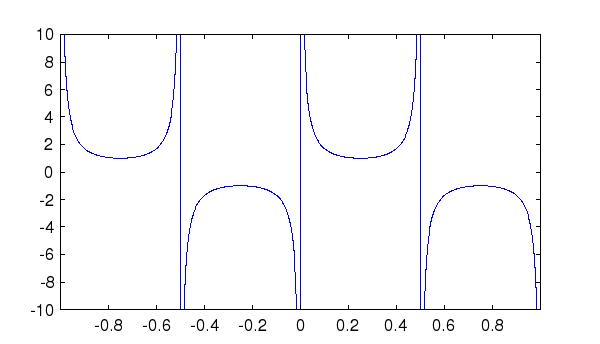
\includegraphics[width=8cm]{cscplot}}

